
% One chapter ---------------------------------------------------------
\chapter*{One}
\addcontentsline{toc}{chapter}{One}

\begin{flushright}
\parbox{0.8\textwidth}{
\emph{God is not external to anyone, but is present with all things, though
they are ignorant that he is so. \\
\hspace*{\fill}{\textperiodcentered \textperiodcentered \textperiodcentered \hspace*{0.2em} Plotinus} } }
\end{flushright}

\noindent
One is chess variant which is played on 26 x 26 board, with white
and dark magenta fields, with light magenta and pink pieces. In
algebraic notation, columns are enumerated from 'a' to 'z', and
rows are enumerated from '1' to '26'. A new piece is introduced,
Starchild.

\clearpage % ..........................................................

\section*{Starchild}
\addcontentsline{toc}{section}{Starchild}

\noindent
\begin{wrapfigure}{l}{0.4\textwidth}
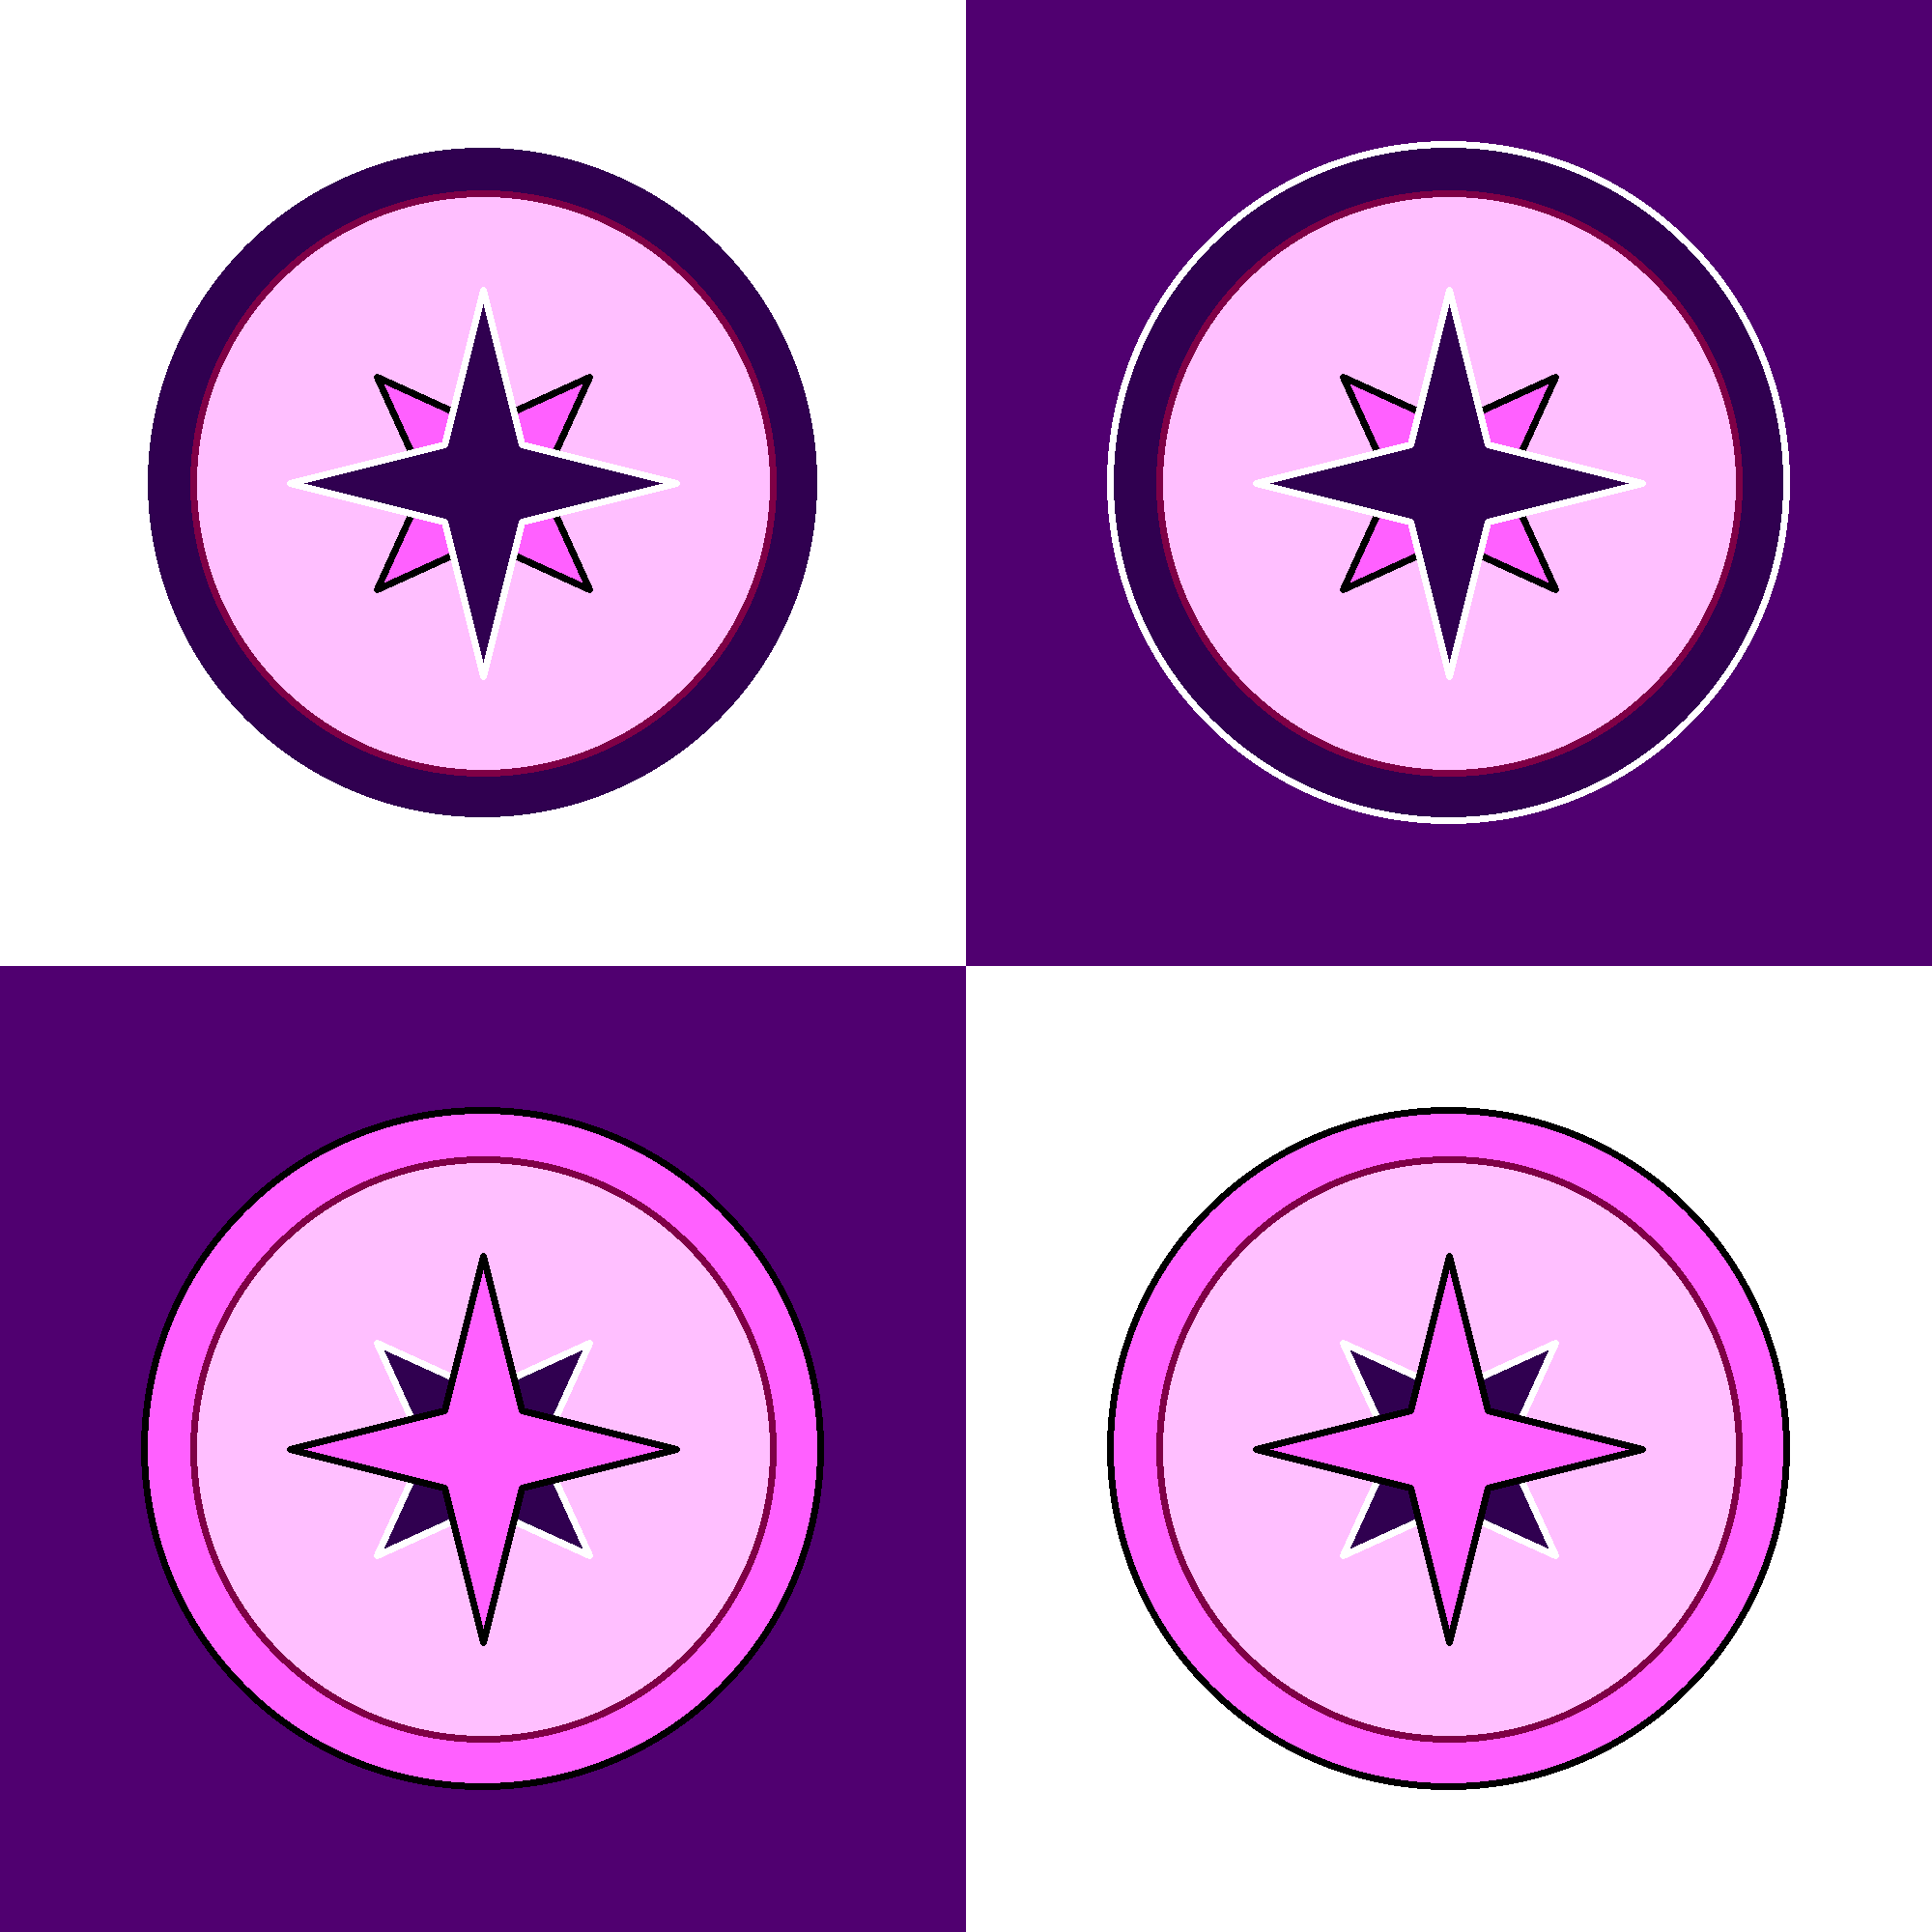
\includegraphics[width=0.4\textwidth, keepaspectratio=true]{pieces/16_starchild.png}
\caption{Starchild}
\label{fig:starchild}
% % \centering
\end{wrapfigure}

\clearpage % ..........................................................

\section*{Initial setup}
\addcontentsline{toc}{section}{Initial setup}

Initial setup can be seen in image below:

\noindent
% \begin{figure}[t]
\begin{figure}[h]
\includegraphics[width=1.0\textwidth, keepaspectratio=true]{boards/22_one.png}
\caption{One board}
\label{fig:one}
% \centering
\end{figure}

\clearpage % ..........................................................
% --------------------------------------------------------- One chapter
